\chapter{Development}
\label{ch.development}

		\todo[inline]{Need a better introducion. vvvv--- this is only copy-paste from proposal.}

	The proposal for this undergraduate dissertation is made up of two main contributions.
	The first contribution will be the port of the \textit{Inter-Cluster Communication Module},
	described in \autoref{sec.inter-cluster-communication}, for the \mppa manycore processor.
	The second contribution will be the design and implementation of communication services
	of a master-slave \os, described in \autoref{sec.communication-services}, on top of
	the inter-cluster communication module.

		\todo[inline]{Insert some paragraphs about the development, tools, etc.}

	\section{\mppa Hardware Resources}
	\label{sec.mppa-hardware-resources}

		A realização da comunicação de baixo-nível depende principalmente de dois recursos do MPPA, interrupções e DMA.
		Primeiro, o sistema de interrupções permitirá a configuração de tratadores das mensagens recebidas e enviadas através da NoC.
		Isto possibilitará a assíncronidade das operações, ponto vital em um sistema operacional baseado no microkernel onde o mestre não pode ficar bloqueado esperando a conclusão de uma única comunicação.
		Caso não fosse possível realizar pelo menos a recebimento de dados/sinais de forma assíncrona, sérios problemas de desempenho seriam introduzidos as camadas superiores.
		Segundo, o DMA é o mediador de todas as comunicações, síncrona ou assíncronas.
		Neste ponto, um hypervisor virtualiza a DMA, separando-a em duas estruturas lógicas globais, uma para a CNoC e outra para a DNoC.
		Cada estrutura agrupa os registradores para a configuração de envio/recebimento, e campos de bits indicando quais slots geraram uma interrupção.
		O hypervisor executa nos RM e controla, de forma assíncrona, as permissões de leitura/escrita dos registradores virtualizados.

		O controle efetuado pelo hypervisor não engloba a alocação ou manipulação dos recursos.
		Consequentemente, nós controlamos manualmente a alocação através de campos de bits.
		Caso uma operação não esteja em conformidade com esse controle, é retornado um valor negativo indicando o erro, \eg alocação de um recursos que já está em uso.
		Assim, não inflingimos custos indesejados ao transferir a responsabilidade de tratar o erro a camada superior, \eg aguardar a liberação do recurso.
		A manipulação envolve procedimentos para configurar a DMA com as devidas permissões e garantir a coerência de cache das operações.
		Por fim, vale ressaltar que não é realizado nenhum controle de concorrência sobre as estruturas comentadas para que não seja inflingido um sobre custo sobre a abordagem do microkernel.
		Caso a HAL seja utilizada para desenvolver um sistema operacional monolítico, o mesmo deve se preocupar em garantir a atômicidade das operações.

		A DMA coordena três linhas de interrupções.
		Duas delas são utilizados pela DNoC para notificar o recebimento de dados e o término do envio dados por uma microthread.
		A CNoC só utiliza uma linha para o recebimento de sinais porque o envio de um sinal, um valor de 64-bits, é realizado explicitamente pelo core.
		Para cada linha de interrupção existe um handler específico mas todos executam um algoritmo similar.
		O Algoritmo 3 exemplifica de forma simplificada o comportamento de um handler.
		Devido ao fato que a linha apenas notifica qual o tipo de interrupção, é responsabilidade do manipulador varrer os recursos de cada interface procurando quem acionou a interrupção.
		Para que não ocorresse a perda de interrupções, foi garantido que o manipulador fosse reentrante.
		Devido ao abordagem do microkernel, os problemas de concorrência são amenizados porque apenas o mestre trata as interrupções.

		\begin{algorithm}
			\caption{Simplified NoC Handler Algorithm.}%
			\label{alg.noc-handler}%
			\begin{algorithmic}[1]
				\Require $status[M_{Interfaces}][N_{Resources}]$, interrupt status of a resource.
				\Require $handlers[M_{Interfaces}][N_{Resources}]$, interrupt handler of a resource.
				\Procedure{noc\_handler}{}
				\For {$i \in [1, M_{Interfaces}]$}
					\For {$j \in [1, N_{Resources}]$}
						\If {$status[i][j] == Interrupt Triggered$}
							\State {$\Call{clean\_status}{i, j}$}
							\State {$\Call{handlers[i][j]}{i, j}$}
						\EndIf
					\EndFor
				\EndFor
				\EndProcedure
			\end{algorithmic}%
			\fonte{Developed by the Author.}%
		\end{algorithm}

		NoC interfaces have two identifiers, one physical (physical ID) and the other logical (logical ID).
		The hardware uses the physical IDs in the process of data routing through \noc.
		Each physical ID is associated with a Logical ID to enable the identification
		of \noc nodes outside the \hal.
		Logical IDs primarily serve to disassociate the node identification from the
		architecture that implements the \hal.
			\autoref{tab.noc-node-id} shows the physical and logical identification performed for \mppa.
		A Tabela 3 apresenta o mapeamento proposto para os clusters do MPPA.
		Cada linha apresenta um dos três grupos de nós NoC existentes (primeira coluna), agrupados por proximidade dos identificadores lógicos.
		Dentro de cada grupo temos um conjunto de identificadores físicos (segunda coluna) que são mapeados 1 para 1 para os identificadores lógicos (terceira coluna).
		Por exemplo, o grupo IO0 constitui 4 interfaces, onde são mapeadas da seguinte forma: $128 \to 0$, $129 \to 1$, $130 \to 2$, e $131 \to 4$.
		A ordem do mapeamento foi definido desta maneira para ficar mais intuitivo qual das interfaces, por consequência o cluster, é o mestre.
		Neste caso, o nó mestre é o identificador lógico 0, IO0.
		Este processo facilita na sincronização após o boot.

		\begin{table}[!tb]
			\centering%
			\caption{NoC Interface Identification.}%
			\label{tab.noc-node-id}%

			\begin{tabular}{l|l|l|}
				\cline{2-3}
									                       & \textbf{Physical ID} & \textbf{Logical ID} \\ \hline
				\multicolumn{1}{|l|}{\textbf{\iocluster0}} & 128-131              & 0-3                 \\ \hline
				\multicolumn{1}{|l|}{\textbf{\iocluster1}} & 192-195              & 4-7                 \\ \hline
				\multicolumn{1}{|l|}{\textbf{\ccluster}}   & 0-15                 & 8-23                \\ \hline
			\end{tabular}

			\fonte{Developed by the Author.}%
		\end{table}

		Para performar a comunicação entre dois clusters, é necessário que o emissor conheça qual o identificador do recurso que o receptor irá usar.
		Por exemplo, caso o receptor configurar o recebimento em um recurso da DNoC e o emissor enviar para outro, mesmo que o identificador lógico esteja correto, o receptor não será notificado do recebimento.
		Por esta razão, os slots de recebimento da CNoC e DNoC foram particionados por abstração.
		Dentro de uma partição, cada slot é mapeado estaticamente para um identificador lógico, \eg 0 à 23.
		Em contraste, os canais de envio não possuem essa necessidade, podendo ser alocados dinâmicamente.
		Entretanto, um conceito importante do Nanvix HAL é prover os recursos necessários para uma determinada operação sem realizar otimizações desnecessárias.
		Desta forma, os canais de envio também foram particionados por abstração de modo que sejam reservados durando toda uma operação.
		A tabela 3 apresenta cada abstração, identificados pelas linhas, e o particionamento dos recursos de cada NoC, identificados pelas colunas.
		Como a abstração sync não realiza a troca de dados arbitrários, não foram reservados recursos na DNoC.
		Vale notar que mesmo com a não utilização de todos os slots existentes, o aperfeiçoamento da programabilidade por não necessitar especificar os recursos de uma comunicação é um ponto forte do design das abstrações.

		% To perform the communication between two clusters, it is necessary that the
		% sender knows which resource the receiver will use.
		% For this reason, the receive slot range of \cnoc and \dnoc are partitioned
		% by abstraction, as can be seen in \autoref{tab.noc-resources}.
		% Within a partition, each slot is associated with a cluster's logical ID.
		% 	\todo{"On the another hand" does not make sense AGAIN.}
		% On the other hand, the transmitters use sending channels that need to
		% be reserved during the entire operation.
		% 	\todo{Explain the table.}
		% Thus, \autoref{tab.noc-resources} also shows the partition of the
		% sending channels for each abstraction.

		\begin{table}[!tb]
			\centering%
			\caption{Partitions of NoC resources by abstraction.}%
			\label{tab.noc-resources}%

			\begin{tabular}{l|l|l|l|l|}
				\cline{2-5}
														& \multicolumn{2}{c|}{\textbf{\cnoc}}          & \multicolumn{2}{c|}{\textbf{\dnoc}}          \\ \cline{2-5}
														& \textbf{RX Slot ID} & \textbf{TX Channel ID} & \textbf{RX Slot ID} & \textbf{TX Channel ID} \\ \hline
				\multicolumn{1}{|l|}{\textbf{\mailbox}} & 0-23                & 0                      & 0-23                & 1-3                    \\ \hline
				\multicolumn{1}{|l|}{\textbf{\portal}}  & 24-47               & 1-2                    & 24-47               & 4-7                    \\ \hline
				\multicolumn{1}{|l|}{\textbf{\sync}}    & 48-71               & 3                      & -                   & -                      \\ \hline
			\end{tabular}

			\fonte{Developed by the Author.}%
		\end{table}

		Por fim, nós conseguimos remover quase toda dependência com a pilha de software disponibilizada pela Kalray.
		Porém, ao eliminar as biliotecas de comunicação, a falta de documentação da virtualização do hardware e exemplos funcionais de comunicação, surgiram limitações no envio dos dados pela DNoC.
		Resumidamente, não foi possível configurar corretamente as microthreads existentes na DMA para envio assíncrono, tornando-se um trabalho futuro.
		Entretanto, tal limitação não impactou no design das abstrações exigindo apenas que o core mestre perca um tempo enviando os dados manualmente.

	\section{Low-Level Communication}
	\label{sec.low-level-comm}

		O Nanvix HAL provê o módulo de comunicação inter-cluster para permitir que cluster distintos troquem informações.
		Esse módulo é constituido de três abstrações, nomeados Sync, mailbox e portal.
		Essas abstrações proveêm mecânismos mais precisos, fáceis de usar, escalonáveis e facilmente portáveis para diferentes arquiteturas~\cite{wentzlaff_fleets:_2011}.
		Sobre eles, é possível criar dos mais simples serviços, como sincronização e troca de dados, à serviços mais complexos como \shm, POSIX Semaphore, \rmem~\cite{penna:rmen}.
		O comportamento esperado pode ser simulado por ambos tipos de chamadas, sincronas ou assíncronas, dependendo apenas do suporte em hardware.
		Motivados a expor melhor controle sobre QoS para as camadas superiores, nós dissociamos as pequenas transferência de dados das grandes, isto é, mailbox e portal.
		Vale notar que seria possível utilizar uma NoC para cada abstração se o hardware suportasse.
		Não fizemos isso no MPPA porque a CNoC só provê a transferência de valores de 64 bits.

		Está seção está organizada da seguinte maneira.
		Subseção 0 abrange pontos comuns entre todas as abstrações.
		Subseção 1, 2 e 3 apresentam conceitualmente cada uma das abstrações, os problemas que elas englobam, e detalhes de implementação.

		\subsection{General Concepts}
		\label{sec.general-concepts}

			Tecnicamente, o Nanvix HAL não sabe que tipos de aplicações ou kernels o utilizaram.
			Desta forma, é preciso garantir um comportamento comum que não afete o funcionanto da camada superior.
			O microkernel, especificamente, restringe o core mestre a estar quase sempre disponível para atender solicitações dos escravos.
			Por isso, as interfaces exportam apenas chamadas assíncronas (isto é, funções async e wait).
			Isto força a camada superior, caso queira, criar chamadas síncronas que chamam a função wait logo após a operação assíncrona.
			Deste modo, no nível do microkernel, nós conseguimos garantir que o mestre configure ou execute as funções assíncronas e notifique os escravos que aguardam na função wait.
			No MPPA, este controle é realizado através de spinlocks atrelados a cada recurso das abstrações.
			Ao concluir uma operação, o mestre libera o bloqueio para o escravo continuar sua execução.

			Contudo, a limitação da DMA descrita na Seção 0 acrescenta um agravante na operação de transferência das abstrações mailbox e portal.
			Nestas abstrações, existe um controle de fluxo onde o receptor deve notificar o emissor, dando-lhe permissão para transferir os dados.
			Este comportamento pode ocasionar o bloqueio do mestre ao esperar uma permissão.
			Para burlar esse problema, foi introduzido o conceito de envio preguiçoso.
			O algoritmo 4 ilustra o comportamento do envio preguiçoso, onde o mestre guarda os paramêtros caso não tenha permissão e vai atender outras solicitações.
			Ao receber a permissão do receptor, o manipulador de interrupções identifica o recurso, realiza de fato o envio dos dados e libera o escravo que solicitou o envio.
			Assim, nós garantimos que o mestre deixe de fazer algo útil e trave todo o sistema.

			\begin{algorithm}
				\caption{Simplified Lazy Transfer Algorithm.}%
				\label{euclid}%
				\begin{algorithmic}[1]
				\Require $resources$, Abstraction Resource Table

				\Algphase{Configures data transfer.}

					\Procedure{async\_write}{$id, message, size$}
						\State {$resources[id].message \gets message$}
						\State {$resources[id].size \gets size$}
						\If {$resources[id].has\_permission$} 
							\State {$\Call{do\_lazy\_write}{id}$}
						\Else
							\State {$resources[id].is\_waiting \gets True$}
						\EndIf
					\EndProcedure%

				\Algphase{Receives permission.}

					\Procedure{abstractions\_handler}{$id$} 
						\If {$resources[id].is\_waiting$} 
							\State {$\Call{do\_lazy\_write}{id}$} 
						\Else
							\State {$resources[id].has\_permission \gets True$}
						\EndIf
					\EndProcedure%

				\Algphase{Transfers the data.}

					\Procedure{do\_lazy\_write}{$id$} 
						\State {$resources[id].is\_waiting \gets False$}
						\State {$resources[id].has\_permission \gets False$}
						\State {$\Call{transfer\_data}{resources[id].message, resources[id].size}$} 
						\State {$\Call{unlock}{resources[id].lock}$}                                \Comment{Releases slave core.}
					\EndProcedure%

				\end{algorithmic}%

				\fonte{Developed by the Author.}%
			\end{algorithm}

			Por fim, as interfaces das abstrações seguem uma convenção para distinguir os papeis de receptor e emissor.
			Receptores utilizam as funções com sufíxo \texttt{create}, \texttt{unlink}, \texttt{aread} e \texttt{wait}.
			Emissores, por sua vez, utilizam funções com sufíxo \texttt{open}, \texttt{close}, \texttt{awrite} e \texttt{wait}.
			Como a função \texttt{wait} é compartilhada, a abstração deve fazer a distinção do papel pelo identificador do recurso.
			A diferenciação da natureza das operações ajuda tanto o usuário, sendo bastante intuitivo, como na implementação da HAL por explicitar quais recursos serão necessário.

			% Por fim, como já comentado anteriormente, o Nanvix HAL não realiza nenhum tipo de multiplexação dos recursos físicos do hardware.
			% A quantidade de recursos de comunicação disponíveis é diretamente relativa a quantidade de recursos físico para realizar uma dada operação.
			% A tabela 4 mostra quais recursos físicos são necessário para cada abstração e a quantidade total de abstrações simultaneas que podem existir.
			% Por exemplo, a criação de um portal precisa de um slot de recebimento da DNoC e 1 canal de transmissão da CNoC.
			% As quantidades são baixas devido aos poucos canais de transmissão, porém quem deve se preocupar com a multiplexação dos recursos deve ser da camada superior.

			% \begin{table}[!tb]
			% 	\centering%
			% 	\caption{Physical requirements by abstraction.}%
			% 	\label{tab.abstractions-amount}%

			% 	\begin{tabular}{l|l|l|l|l|l|l|}
			% 		\cline{2-7}
			% 												& \multicolumn{3}{c|}{\textbf{Create}}  & \multicolumn{3}{c|}{\textbf{Open}}                              \\ \cline{2-7}
			% 												& \multicolumn{1}{|c|}{\textbf{RX}}
			% 												            & \multicolumn{1}{|c|}{\textbf{TX}}
			% 															            & \multicolumn{1}{|c|}{\textbf{Available}}
			% 																		                & \multicolumn{1}{|c|}{\textbf{RX}}
			% 																				                    & \multicolumn{1}{|c|}{\textbf{TX}}
			% 																				        			            & \multicolumn{1}{|c|}{\textbf{Available}} \\ \hline
			% 		\multicolumn{1}{|l|}{\textbf{\mailbox}} & 1 (\dnoc) & 1 (\cnoc) & 1             & 1 (\cnoc) & 1 (\dnoc) & 4                                        \\ \hline
			% 		\multicolumn{1}{|l|}{\textbf{\portal}}  & 1 (\dnoc) & 1 (\cnoc) & 2             & 1 (\cnoc) & 1 (\dnoc) & 4                                        \\ \hline
			% 		\multicolumn{1}{|l|}{\textbf{\sync}}    & 1 (\cnoc) & 0         & 24            & 0         & 1 (\cnoc) & 1                                        \\ \hline
			% 	\end{tabular}

			% 	\fonte{Developed by the Author.}%
			% \end{table}

		\subsection{Sync Abstraction}
		\label{sec.sync-abs}

			A abstração de sincronização, chamada sync, provê o básico para a sincronização de clusters.
			A partir dela, é possível criar barreiras distribuidas.
			Seu comportamento é análogo a abstração POSIX Signals, mas as notificações não carregam informações, servem apenas para sincronização.
			O sync define dois modos de sincronização, ALLTOONE e ONETOALL.
			Nois dois modos, os clusters são separados entre um único nó mestre (ONE) e um ou mais nós escravos (ALL).
			A Figura 1 ilustra o modo ALLTOONE, onde o nó mestre aguarda bloqueado os N escravos realizarem a sincronização.
			Em contrapartida, o modo ONETOALL mostra o mestre notificando os N escravos, liberando-os do bloqueio, ilustrado pela Figura 3.
			Os nós emissores nunca ficam bloqueados, o trabalho deles é emitir um sinal.
			Os nós receptores são responsáveis por aguardar a chegada de todas as notificações.

			\begin{figure}[!tb]
				\centering%
				\caption{Synchronization Abstraction Example.}%
				\label{fig:sync-concepts}%

				\subcaptionminipage[fig:sync-all-to-one]%
					{.6\linewidth}%
					{N Slaves notify the Master (\texttt{ALL\_TO\_ONE}).}%
					{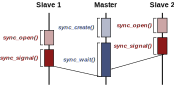
\includegraphics[width=\linewidth]{sync-all-to-one.pdf}}%
				\hfill
				\subcaptionminipage[fig:sync-one-to-all]%
					{.6\linewidth}%
					{The Master notify N Slaves (\texttt{ONE\_TO\_ALL}).}%
					{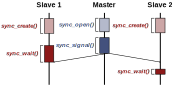
\includegraphics[width=\linewidth]{sync-one-to-all.pdf}}%

				\fonte{Developed by the Author.}%
			\end{figure}

			\subsubsection{Receiver Side Implementation}

				O Codigo 4 apresenta a interface do Sync proposta para o Nanvix HAL.
				Como mencionado na Seção (recursos de hardware), é possível identificar os dois conjuntos de funções, um para os receptores e outro para emissor.

\begin{listing}[!tb]
\caption{Nanvix HAL: Sync Interface for Receiver.}
\label{code:hal-sync-receiver}
\begin{minted}{c}
/**
 * @brief Allocates and configures the receiving side of
 * the synchronization point.
 */
int sync_create(const int *nodes, int nnodes, int type);

/* @brief Releases and cleans receiver slot. */
int sync_unlink(int syncid);

/* @brief Waits a signal. */
int sync_wait(int syncid);
\end{minted}
\fonte{Developed by the Author.}
\end{listing}

			\subsubsection{Sender Side Implementation}

				Ela foi pensada para que os parâmetros de criação fossem os mesmo que os parâmetros de abertura.

\begin{listing}[!tb]
\caption{Nanvix HAL: Sync Interface for Sender.}
\label{code:hal-sync-sender}
\begin{minted}{c}
/**
 * @brief Allocates and configures the sending side of
 * the synchronization point.
 */
int sync_open(const int *nodes, int nnodes, int type);

/* @brief Releases the transfer channel. */
int sync_close(int syncid);

/* @brief Sends a signal. */
int sync_signal(int syncid);
\end{minted}
\fonte{Developed by the Author.}
\end{listing}

		\subsection{Mailbox Abstraction}
		\label{sec.mailbox-abs}

			\begin{figure}[!tb]
				\centering%
				\caption{Mailbox Abstraction Concept.}%
				\label{fig:conpt_mailbox}%

				\subcaptionminipage[fig:conpt_mailbox-logical]%
					{.5\linewidth}%
					{Conceptual Overview.}%
					{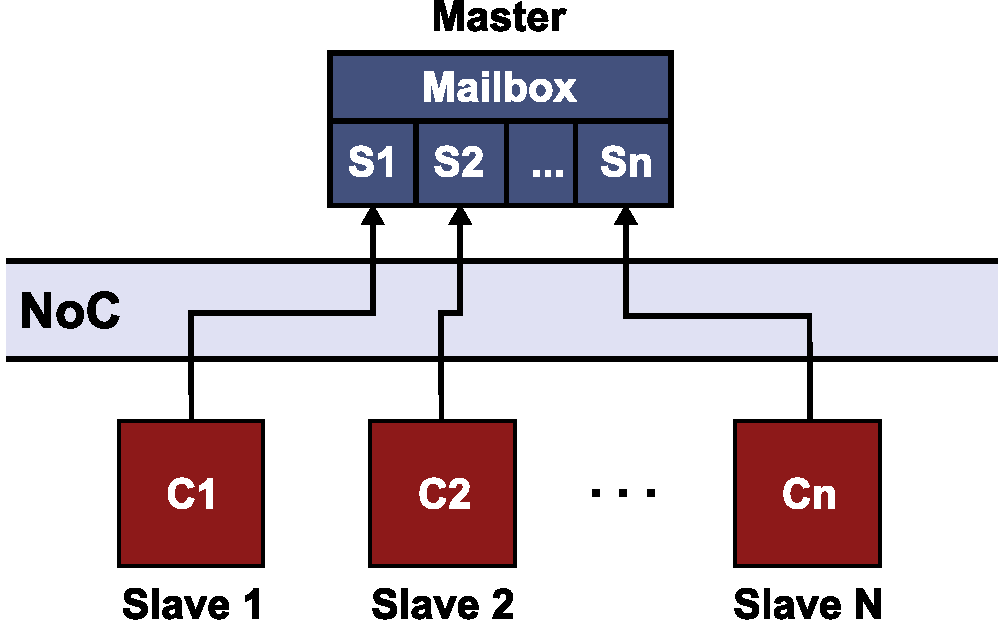
\includegraphics[width=\linewidth]{mailbox-logical.pdf}}%

				\hfill

				\subcaptionminipage[fig:conpt_mailbox-flow]%
					{.6\linewidth}%
					{Flow of execution: Slave sends a message, Master reads and notifies the sender.}%
					{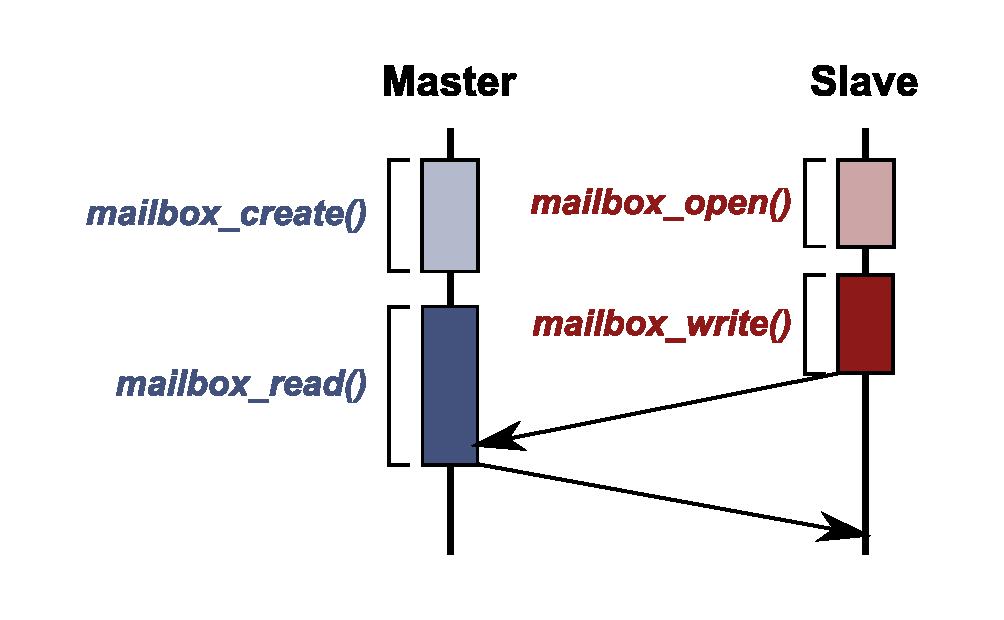
\includegraphics[width=\linewidth]{mailbox-flow.pdf}}%

				\fonte{Developed by the Author.}%
			\end{figure}

				\todo[inline]{Make it more detailed.}

			The \textit{Mailbox Abstraction} allows clusters to exchange fixed-size
			messages with each other.
			The message was thought to be a relatively small size, usually a few hundred bytes.
			Similarly, the operation of the \mailbox follows \posix message queue behavior.
			For example, the message can be used to encode small operations and system
			control signals.
			As illustrated in \autoref{fig:conpt_mailbox}, the operation cardinality is N:1,
			where N senders can transfer one message at a time to a receiver queue.
			When the receiver consumes a message, it notifies the sender to ensure
			control of the flow.

			\subsubsection{Receiver Side Implementation}

\begin{listing}[!tb]
\caption{Nanvix HAL: Mailbox Interface for Receiver.}
\label{code:hal-mailbox-receiver}
\begin{minted}{c}
/* @brief Creates a mailbox. */
int mailbox_create(int nodenum);

/* @brief Destroys a mailbox. */
int mailbox_unlink(int mbxid);

/* @brief Reads data from a mailbox. */
ssize_t mailbox_aread(int mbxid, void * buffer, size_t size);

/**
 * @brief Waits for an asynchronous operation on a
 * mailbox to complete.
 */
int mailbox_wait(int syncid);
\end{minted}
\fonte{Developed by the Author.}
\end{listing}

			\subsubsection{Sender Side Implementation}

\begin{listing}[!tb]
\caption{Nanvix HAL: Mailbox Interface for Sender.}
\label{code:hal-mailbox-sender}
\begin{minted}{c}
/* @brief Opens a mailbox. */
int mailbox_open(int nodenum);

/* @brief Closes a mailbox. */
int mailbox_close(int mbxid);

/* @brief Writes data to a mailbox. */
ssize_t mailbox_awrite(int mbxid, const void * buffer, size_t size);

/**
 * @brief Waits for an asynchronous operation on a
 * mailbox to complete.
 */
int mailbox_wait(int syncid);
\end{minted}
\fonte{Developed by the Author.}
\end{listing}

				As explained in \autoref{sec.mailbox-abs}, the \mailbox abstraction
				allows the exchange of small messages of sizes between clusters similar
				to a \posix message queue.
				The \mailbox is more complex than the previous abstraction because it
				uses both \dnoc and \cnoc resources.
				When executing the function \texttt{mailbox\_create()}, the receiver
				will only use one \dnoc receive slot and configures it with a kernel
				memory space, sufficient to receive 24 messages.
				The messages are composed of the header identifying the sender
				and a body containing the useful message.
				When consuming a message (\texttt{mailbox\_read()}), the receiver
				will copy the message to the user's buffer and send a signal
				to the sender informing him that it can send another message.
				If there is no message in the buffer, the receiver is blocked
				until a message is received.

					\todo{"On the another hand" does not make sense AGAIN.}
				On the other hand, the sender will allocate a receive signal slot (\texttt{mailbox\_open()})
				before sending its first message to the receiver.
				If the sender attempts to send a message before the receiver has consumed
				the previous message, the sender will be blocked waiting for the sender's notification.
				In this way, flow control is guaranteed, and the sender will not overwrite
				messages unread by the receiver.
				Sending the message will always be executed asynchronously
				because it will always be necessary to copy the message to
				a kernel buffer that contains the header.
				Thus, the sender will never be blocked waiting for the message to be sent.
				In this configuration, the number of mailbox creations (\texttt{mailbox\_create()})
				within a cluster is limited to 1 because of the \cnoc sending channel.
					\todo{"On the another hand" does not make sense AGAIN.}
				On the other hand, the maximum number of opens (\texttt{mailbox\_open()}) is
				4 because of the limitation of the available \dnoc sending channels.

		\subsection{Portal Abstraction}
		\label{sec.portal-abs}

			\begin{figure}[!tb]
				\centering%
				\caption{Portal Abstraction Concept: Node 1 create a portal and notify Node 2 to transfer the data.}%
				\label{fig:conpt_portal}%
				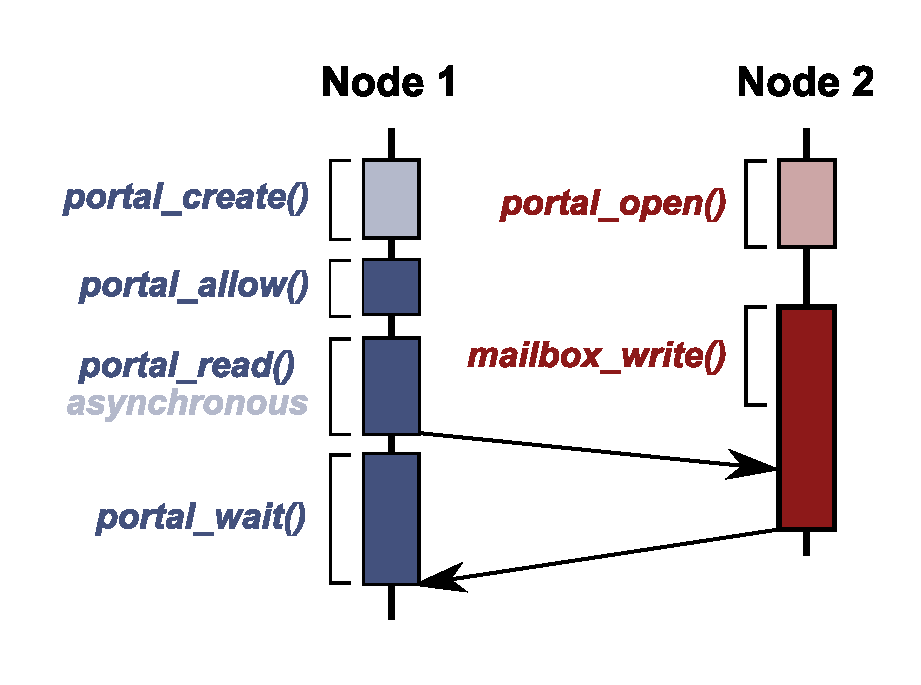
\includegraphics[width=.65\textwidth]{portal.pdf}%
				\fonte{Developed by the Author.}%
			\end{figure}

				\todo[inline]{Make it more detailed.}

			Lastly, the \textit{Portal Abstraction} enables two clusters to exchange arbitrary
			amounts of data.
			The conceptual idea of the \portal is similar to that implemented in \posix pipes.
			\autoref{fig:conpt_portal} shows the \portal operation, with cardinality
			1:1, a cluster pair opens a channel to transfer data.
			However, the operation is only allowed in one direction with a flow control mechanism,
			where the receiver cluster warns the sender cluster when it is ready to receive.

			\subsubsection{Receiver Side Implementation}

\begin{listing}[!tb]
\caption{Nanvix HAL: Portal Interface for Receiver.}
\label{code:hal-portal-receiver}
\begin{minted}{c}
/* @brief Creates a portal. */
int portal_create(int local);

/* @brief Destroys a portal. */
int portal_unlink(int portalid);

/* @brief Allow sender to transfer data. */
int portal_allow(int portalid, int remote);

/* @brief Reads data asynchronously from a portal. */
ssize_t portal_aread(int portalid, void * buffer, size_t size);

/**
 * @brief Waits for an asynchronous operation on a
 * portal to complete.
 */
int portal_wait(int portalid);
\end{minted}
\fonte{Developed by the Author.}
\end{listing}

			\subsubsection{Sender Side Implementation}

\begin{listing}[!tb]
\caption{Nanvix HAL: Portal Interface for Sender.}
\label{code:hal-portal-sender}
\begin{minted}{c}
/* @brief Opens a portal. */
int portal_open(int remote);

/* @brief Closes a portal. */
int portal_close(int portalid);

/* @brief Writes data asynchronously to a portal. */
int portal_awrite(int portalid, const void * buffer, size_t size);

/**
 * @brief Waits for an asynchronous operation on a
 * portal to complete.
 */
int portal_wait(int portalid);
\end{minted}
\fonte{Developed by the Author.}
\end{listing}

				\autoref{sec.portal-abs} showed that the portal abstraction is similar to
				a \posix pipe with flow control.
				So, the \portal analogously follows the ideas implemented
				in the \mailbox with the difference of the option to write,
				that can be synchronously or asynchronously.
				The total number of receive data operations (\texttt{portal\_create()})
				is limited to 2 because of the number of available signal sending channels.
					\todo{"On the another hand" does not make sense AGAIN.}
				On the other hand, up to 4 send operations (\texttt{portal\_open()})
				can be performed simultaneously because there are 4 available send
				channels for the \portal.

				Function \texttt{portal\_open()} starts the data send operation.
				In it will be allocated a channel of data sending associated with
				a $\mu$thread.
				Also, a signal receiving slot will be allocated to receive the
				signal that will release the sender to transfer data to the receiver.
				In asynchronous send operation (\texttt{portal\_awrite()}), the cluster
				cannot modify or release the buffer until the operation is completed.
				To ensure that the buffer can use, the cluster must call function \texttt{portal\_wait()}.

				The receiver will allocate a receiving slot of the \dnoc and a transfer
				channel (\texttt{portal\_create()}) to receive data from another cluster.
				After setting up the resources (\texttt{portal\_read()}), the receiver
				can notify a sender (\texttt{portal\_allow()}), enabling it to transfer data.
				For this reason, the read operation is always performed asynchronously.
				After receiving the set amount of data, the receiver can use the buffer securely.

	
	\section{User-Level Communication}
	\label{sec.comm-services}

		\subsection{Inter-Cluster Communication Services}
		\label{sec.inter-cluster-communication-module}

			The inter-cluster communication module, described in \autoref{sec.inter-cluster-communication-module},
			is designed to export a standard and straightforward communication
			primitives to different lightweight manycores.
			These primitives can be used by various types of operating systems
			and applications.
			Thus, the module is flexible enough not to impact the performance
			of the upper layers negatively.
			For this, it does not provide rich management of the exposed abstractions.

			In this scenario, the communication services of Nanvix Microkernel seek
			to provide \ipc between distinct clusters.
			Specifically, these services perform the multiplexing of the hardware
			resources and the verification of the parameters that will be passed
			on the communication primitives.
			Due to the Master-Slave model, the responsibility of protecting,
			manipulating, and configuring \hal resources is of the master core.
			The slave core will request operations through a meta-interface,
			passing the necessary information to the master.

			Considering that the abstractions make up the fundamental elements of
			the construction of more complex services, the Microkernel services
			were responsible for the management and multiplexing of the finite
			resources for the many cores of a cluster.
			In total, there are three communication services in the Nanvix Microkernel,
			each associated with an abstraction of the communication module,
			analogously named \sync, \mailbox, and \portal services.

		\subsection{Inter-Cluster Communication Services Implementation}

			\todo[inline]{Temporary}

			As described in \autoref{sec.communication-services}, three communication
			services will be developed for the Nanvix Microkernel, named \sync, \mailbox,
			and \portal services.
			Each service will be responsible for protecting, managing, manipulating,
			and multiplexing the resources exposed by the \hal communication module.
			These services must take into account the memory constraints and the
			master-slave model chosen for the Microkernel.

			Management and manipulation operations are similar to all services.
			They will be provided through interfaces that function as wrappers
			for the \hal abstraction functions.
			In the implementation of these interfaces, there will be a mapping
			between low-level identifiers, associated with \hal resources,
			and high-level identifiers, associated with resource protection structures.

			\todo[inline]{
				According to Odorico, for the completion of the work, it is important to highlight:
				\\ - How do you treat the protection operations?
				\\ - How do you intend to test and to validate the correctness of the implemented services.
			}

			The protection operations are mostly similar.
			For instance, the use of unallocated resources, sanitizing entries,
			checking valid identifiers, non-null pointers, and checking
			for conflicting operations (reading in write-only resources).
			In the meantime, there are exceptional cases in some services
			that must be taken.
			For instance, in the \sync service, a cluster cannot synchronize
			with itself, or there is a repetition of identifiers in the
			stipulated set of clusters.

			Finally, some aspects of services and implementation still need
			to be analyzed and will be better detailed in another version
			of the dissertation.
			For example, what resource multiplexing methods will be used
			and their impacts on the Nanvix Microkernel services.